\section{Introduction}
\subsubsection{Discretization \& Linearization}
{\small
\noindent
\begin{minipage}[t]{0.32\linewidth}

\textbf{Euler Discretization}\\
\begin{align*}
x(k) &= x^c(t_0 + kT_s)\\
u(k) &= u^c(t_0 + kT_s)\\
A &= \mathbb{I} + T_sA^c\\
B &= T_s B^c\\
C &= C^c\\
D &= D^c
\end{align*}
\end{minipage}%
\hfill
\begin{minipage}[t]{0.32\linewidth}

\textbf{Exact Discretization}\\
\begin{align*}
A &= \exp{(A^c \cdot T_s)}\\
B &= \int^{T_s}_0 \exp{(A^c \cdot \tau)}\, d\tau\, B^c\\
C &= C^c\\
D &= D^c
\end{align*}
If $A^c$ invertible:\\
$B = (A^c)^{-1}(A-\mathbb{I})B^c$
\end{minipage}%
\hfill
\begin{minipage}[t]{0.32\linewidth}
\textbf{Linearization (Taylor)}\\
Around $\bar{x},\bar{u}$ (first order):\\
\[
f(\bar{x}) + \frac{\partial f}{\partial x^\top}\Big|_{\bar{x}} \cdot (x-\bar{x})
\]

\vspace{-0.5em}
\begin{align*}
\dot{x} &= \underbrace{\tfrac{\partial g}{\partial x^\top}}_{A^c} \delta x + \underbrace{\tfrac{\partial g}{\partial u^\top}}_{B^c} \delta u\\[0.3em]
y &= \underbrace{\tfrac{\partial h}{\partial x^\top}}_{C} \delta x + \underbrace{\tfrac{\partial h}{\partial u^\top}}_{D} \delta u
\end{align*}
\end{minipage}

\vspace{0.3em}
\noindent\textbf{Exact Solution}\\
$x(t) = e^{A^c(t-t_0)}x_0 + \displaystyle\int_{t_0}^{t} e^{A^c(t-\tau)}B^c u(\tau)\,d\tau \qquad e^{A^ct} := \sum_{n=0}^{\infty}\frac{(A^ct)^n}{n!}$
}


% \subsection{Analysis of LTI Discrete-Time Systems}
% \subsubsection{Coordinate Transformation}
% Consider the linear transformation $\tilde{x}(k) = Tx(k)$ with $\det(T) \neq 0$ (invertible):

% \begin{align*}
%     \tilde{x}(k+1) &= \underbrace{TAT^{-1}}_{\tilde{A}} \tilde{x}(k) + \underbrace{TB}_{\tilde{B}} u(k) \\
%     y(k) &= \underbrace{CT^{-1}}_{\tilde{C}} \tilde{x}(k) + \underbrace{D}_{\tilde{D}} u(k)
% \end{align*}

% \subsubsection{Stability}
% The LTI system $x(k+1) = Ax(k)$ is:

% \begin{itemize}[leftmargin=*]
%     \item \textbf{Marginally Stable:} If all eigenvalues $|\lambda_j| \leq 1$, and those with $|\lambda_j| = 1$ have a geometric multiplicity equal to their algebraic multiplicity. The state remains bounded.
    
%     \item \textbf{Globally Asymptotically Stable (GAS):} If all eigenvalues $|\lambda_j| < 1$ (inside the open unit circle). This implies $\lim_{k \to \infty} x(k) = 0$.
    
%     \item \textbf{Unstable:} If at least one eigenvalue $|\lambda_j| > 1$, or if there are eigenvalues on the unit circle with a geometric multiplicity less than their algebraic multiplicity.
% \end{itemize}

\subsubsection{Controllability and Observability}
The LTI system is \textbf{controllable} if the controllability matrix 
$\mathcal{C} = [B \quad AB \quad \dots \quad A^{n-1}B]$ has $\text{rank}(\mathcal{C}) = n$. 
\\ \textbf{Controllability} $\implies$ \textbf{Stabilizability}. A system is stabilizable if all uncontrollable modes (eigenvalues) are asymptotically stable ($|\lambda_j| < 1$).

\vspace{2pt}
The LTI system is \textbf{observable} if the observability matrix 
$\mathcal{O} = [C^\top \quad (CA)^\top \quad \dots \quad (CA^{n-1})^\top]^\top$ 
has $\text{rank}(\mathcal{O}) = n$. 
\\ \textbf{Observability} $\implies$ \textbf{Detectability}. A system is detectable if all unobservable modes are asymptotically stable ($|\lambda_j| < 1$).


\subsubsection{Stability of Nonlinear Systems}

An equilibrium $\bar{x}$ is \textbf{Lyapunov stable} if $\forall\,\epsilon>0\;\exists\,\delta(\epsilon)>0$ such that
$\|x(0)-\bar{x}\|<\delta(\epsilon) \Rightarrow \|x(k)-\bar{x}\|<\epsilon\;\forall k\ge0$,
and \textbf{globally asymptotically stable (GAS)} if additionally $\|x(k)-\bar{x}\|\to 0$ as $k\to\infty$ for all $x(0)\in\mathbb{R}^n$.

A \textbf{Lyapunov function} $V$ is GAS of $\bar{x}=0$ if:
$V(0)=0$, $V(x)>0$ and $V(x)\to\infty$ for all $x\neq 0$, and $V(g(x))-V(x)\le-\alpha(x)\le0\;\forall x$.
If $\alpha(x)$ is only positive \emph{semi}definite, then $\bar{x}$ is globally Lyapunov stable.

\textbf{Indirect Method}: Let $A=\left.\frac{\partial g}{\partial x^T}\right|_{x=0}$.
The origin is locally asymptotically stable if $|\lambda_i|<1\;\forall i$, and unstable if $|\lambda_i|>1$ for some $i$.
If any $|\lambda_i|=1$, no conclusion can be drawn.

\textbf{Linear Systems}: With $V(x)=x^TPx$ and the discrete-time Lyapunov equation $A^TPA-P=-Q$,
a unique solution $P>0$ exists for some $Q>0$ \emph{iff} all eigenvalues of $A$ lie strictly inside the unit circle.
Hence, for LTI systems, GAS is both necessary and sufficient and always global.

\subsection{LQR}
Valid for \textbf{LTI} systems $x(k+1) = Ax(k) + Bu(k)$ with \textbf{quadratic cost function}:
\begin{equation}
\label{LQR}
    J(x_0, U) = x_N^TPx_N + \sum_{i=0}^{N-1}x_i^TQx_i + u_i^TRu_i
\end{equation}
We regulate the state to the origin ($x=0$) and we have \textbf{no} constraints.
$P = P^T $ is the \textbf{terminal} weight $ P \succeq 0$.
$Q = Q^T $ the \textbf{state} weight $ Q \succeq 0$  and  $R = R^T $ is the \textbf{input} weight $ R \succ 0$. $x(0)$ is the current state, $x_0, \dots, x_N$ and $u_0, \dots, u_N$ the optimization variables.

\subsubsection{Batch approach}
Results in a series of numerical values based on the initial state $x(0)$.
\begin{center}
    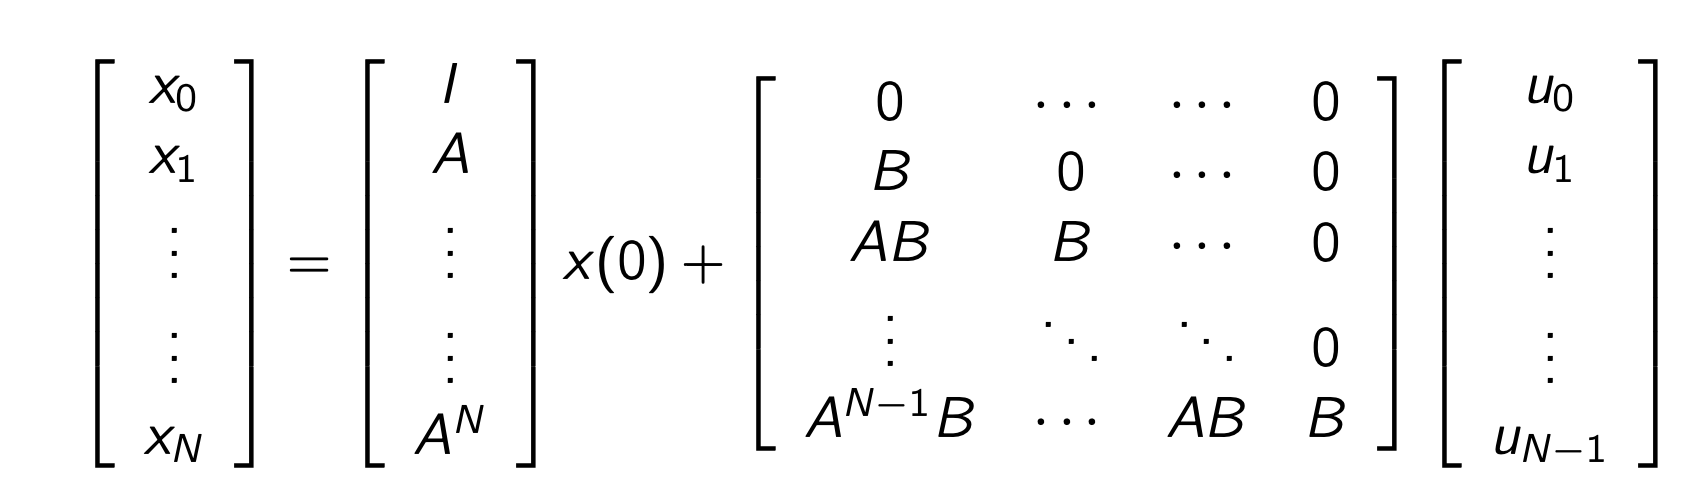
\includegraphics[width=0.6\linewidth]{images/batch.png}
\end{center}

Or in compact notation as $X = S^x x(0) + S^uU$ and with $\Bar{Q} = \text{blockdiag}(Q, \cdots, Q, P)$ , $\Bar{R} = \text{blockdiag}(R, \cdots, R)$. 
The cost function becomes:
\begin{align*}
J(x(0), U)  &= X^T\Bar{Q}X + U^T\Bar{R}U \\
&= U^THU + 2x(0)^TFU + x(0)^TS^{xT}\Bar{Q}S^xx(0)
\end{align*}
with $ H = (S^u)^T\Bar{Q}S^u + \bar{R}$ and $F = (S^x)^T\Bar{Q}S^u$. Note that $H \succ 0$. Minimizing $\nabla_U J(x(0), U) = 0$:

\begin{tcolorbox}[eqbox]
\begin{align*}
U^\star &= -H^{-1}F^Tx(0) \\
J^\star &= -x(0)^TFH^{-1}F^Tx(0) + x(0)^T(S^x)^T\Bar{Q}S^xx(0)
\end{align*}
\end{tcolorbox}

\subsubsection{Recursive approach}
From (\ref{LQR}) we start solving for time $N-1$, obtaining the recursive formula:

\begin{tcolorbox}[eqbox]
\begin{align*}
u_i^\star &= -(B^TP_{i+1}B + R)^{-1}B^TP_{i+1}Ax(i) = F_{i}x_{i} \\
P_i &= A^TP_{i+1}A + Q \\
    &\quad - A^TP_{i+1}B(B^TP_{i+1}B + R)^{-1}B^TP_{i+1}A \\
J^\star_{i}(x(i)) &= x(i)^TP_ix(i)
\end{align*}
\end{tcolorbox}
\textbf{Batch} vs \textbf{Recursive}: batch adapts more easily to constraints; recursive is more efficient and robust to uncertainties.

\textbf{ARE} ($N\to\infty$): steady-state $P_\infty$, $F_\infty = -(B^TP_\infty B+R)^{-1}B^TP_\infty A$
\begin{itemize}[leftmargin=*]
    \item $u^\star(k) = F_\infty x(k)$ $\Rightarrow$ closed loop \textbf{asymptotically stable}
    \item $J^\star = x^TP_\infty x$ is a \textbf{Lyapunov function} of $x(k+1)=(A+BF_\infty)x(k)$
\end{itemize}

\subsection{Convex Optimization}
The standard form is:
\begin{equation} \label{eq:opt_standard_form}
\begin{aligned}
\min_{x \in \text{dom}(f)} \quad & f(x) \\
\text{subj. to} \quad & g_i(x) \leq 0 \\
& h_i(x) = 0 
\end{aligned}
\end{equation}
The $i^{th}$ inequality constraint $g_i(x) \leq 0$ is active at $\Bar{x}$ if $g_i(\Bar{x}) = 0$, otherwise it is inactive. Equality constraints are always active. 
\subsubsection{Convex Sets}
A set is a \textbf{convex set} if and only if for $x$ and $y$ $\in \mathcal{X}$:
\begin{center}
    $\lambda x + (1-\lambda)y \in \mathcal{X}, \forall \lambda \in [0,1], \forall x, y \in \mathcal{X}$
\end{center}

\begin{enumerate}
    \item \textbf{Hyperplane}: Defined as $a^Tx = b$ (\textit{affine}).
    \item \textbf{Halfspace}: $a^Tx \leq b$ Everything on one side of the Hyperplane.
    \item \textbf{Polyhedron}:  $Ax \leq b$ Intersection of a finite number of closed halfspaces.
    \item \textbf{Polytope}: A bounded polyhedron.
    \item \textbf{Ellipsoid}: $(x-x_c)^TA^{-1}(x-x_c) \leq 1$ with $x_c$ the center and $A \succ 0$.
    \item \textbf{Norm Balls}: $ \| x - x_c \|_p \leq r$ with a radius $r$ and a norm $p$
\end{enumerate}
\textbf{The intersection of two or more convex sets is itself convex.} (Union not convex in general)

\subsubsection{Convex Functions}
A function is convex iff dom(f) is convex and $f(\lambda x + (1-\lambda)y) \leq \lambda f(x) + (1-\lambda)f(y)$.
\begin{enumerate}
    \item \textbf{First-order condition}: convex iff $f(y) \geq f(x) + \nabla f(x)^T(y-x)$
    \item \textbf{Second-order condition}: convex iff $\nabla^2f(x) \succeq 0$
\end{enumerate}
\begin{itemize}
    \item \textbf{Affine}: $ax + b$ for any $a,b \in \mathbb{R}$
    \item \textbf{Exponential}: $e^{ax}$ for any $a \in \mathbb{R}$
    \item \textbf{Powers}: $x^\alpha$ on $\mathbb{R}_{++} \text{ and } \alpha \geq 1 \text{ or } \alpha \leq 0$
    \item \textbf{Vector norms}: $\|x\|_p$ for $p \geq 1$
\end{itemize}

\textbf{Operations that preserve convexity}: Non-negative weighted sum, Composition with affine function, Pointwise maximum or supremum, Partial minimization,...

\subsubsection{Optimality Conditions}
For a convex problem of the form (\ref{eq:opt_standard_form}), the \textbf{Lagrangian Function} is defined as $L(x, \lambda, \nu) = f(x) + \sum_{i =1}^m \lambda_i g_i(x) + \sum_{i =1}^p \nu_i h_i(x)$ The \textbf{dual function} is defined as $d(\lambda,\nu) = \inf_x L$, it is  \textbf{always concave} and generates a \textbf{lower bound} $d(\lambda, \nu) \leq p^\star$. The dual problem $ d^\star = \max d(\lambda, \nu)$ subject to $\lambda \geq 0$ is \textbf{always convex} even if the primal is not.\vspace{4pt}

If there is at least one strictly feasible point (for convex problems), then $p^\star = d^\star$ (\textbf{Slater Condition}). Moreover the \textbf{KKT conditions} are defined as
\begin{enumerate}
    \item \textbf{Stationarity}: $\nabla_x L = \nabla f(x^\star)+ \sum \lambda_i^\star \nabla g_i(x^\star) + \sum\nu_i^\star \nabla h_i(x^\star) = 0$
    \item \textbf{Primal Feasibility}: $h_i(x^\star) = 0$ and $g_i(x^\star) \leq 0$
    \item \textbf{Dual Feasibility}: $\lambda^\star \geq 0$
    \item \textbf{Complementarity Slackness}: $\lambda^\star_i g_i(x^\star)= 0$
\end{enumerate}
For Convex with Slatter condition they are \textbf{necessary and sufficient}, but in general just \textbf{necessary}.

\subsubsection{Sensitivity Analysis}

\[
\begin{array}{@{}c@{\qquad}|@{\qquad}c@{}}
    \begin{aligned}
        \min_{x} \quad & f(x) \\
        \text{subj. to} \quad & g_i(x) \le u_i \quad i=1\ldots m \\
        & h_i(x) = v_i \quad i=1\ldots p,
    \end{aligned}
    &
    \begin{aligned}
        \max_{\nu, \lambda} \quad & d(\nu, \lambda) - u^\top \lambda - v^\top \nu \\
        \text{subj. to} \quad & \lambda \ge 0
    \end{aligned}
\end{array}
\]

Assuming strong duality for the original unperturbed problem, weak duality for the perturbed case implies:
\[
    p^\star(u,v) \ge d^\star(\nu^\star, \lambda^\star) - u^\top\lambda^\star - v^\top\nu^\star = p^\star(0,0) - u^\top\lambda^\star - v^\top\nu^\star
\]

\begin{itemize}
    \item \textbf{Global Sensitivity:} Evaluated by varying $\lambda_i^\star, \nu_i^\star$ and $u_i, v_i$.
    
    \item \textbf{Local Sensitivity:} If $p^\star(u, v)$ is differentiable at $(0, 0)$, then:
    \[
        \lambda_i^\star = -\frac{\partial p^\star(0, 0)}{\partial u_i}, \qquad \nu_i^\star = -\frac{\partial p^\star(0, 0)}{\partial v_i}
    \]
    \begin{itemize}
        \item $\lambda_i^\star$ is the sensitivity of $p^\star$ relative to the $i^{\text{th}}$ inequality.
        \item $\nu_i^\star$ is the sensitivity of $p^\star$ relative to the $i^{\text{th}}$ equality.
    \end{itemize}
\end{itemize}

\vspace{2.5em}